\section{Method}
    The algorithms presented are implemented and simulated in python using several libraries. Some of these have functions which are implemented explicitly; the PCA is for example implemented using a package from the scikit-learn library. This will be gone into further detail later on. Before building the neural network, the data must be prepared. This is called preprocessing.
    \subsection{Preprocessing of the Data Set}
        The most important section of any data analysis is getting to know and performing a preprocessing of the data set. This involves formating the data in a manner which is easily interpreted and understood by the neural network nodes. Firstly, an outlier filtration is performed on the data.
        \subsubsection{Outlier Filtration}
            Outlier filtration involves removing data which does not belong in the dataset. Data which is out of the defined boundaries can often be found in large datasets which are input by people, as is likely to be case for the credit card data presented. There are a few defined boundaries of the data which are easy to filter out. This is for example the gender definition made by the bank, where 1=male and 2=female. This automatically excludes all values outside of this definition.\\\\
            The definitions presented are:
            \begin{itemize}
                \item X1: Amount of given credit. Must be positive.
                \item X2: Gender (1=male, 2=female)
                \item X3: Education (1=graduate school, 2=university, 3=highschool, 4=other).
                \item X4: Marital Status (1=married, 2=single, 3=others)
                \item X5: Age
                \item X6 - X11: History of past payment. Can be any integer from -2 to 9.
                \item X12-X17: Amount of bill statement. Can be negative.
                \item X18-X23: Amount of previous payment. Must be positive.
            \end{itemize}
            Before any scaling is applied, these categorical outliers are removed.
        \subsubsection{Column Scaling}
            Some of the columns have values which require scaling before they are input into the network. If the data were not scaled in the preprocessing, then the sigmoid activation function of the age (values from 20 upwards) would just result in values which are very close to one. The network would not be able to distinguish between these values as well as it would if the ages were centered around 0 with a standard deviation of one (the typical way to scale). In this case, the 'resolution' of the sigmoid (or similar functions such as the hyperbolic tangent) would be far better, resulting in a network which can tell the difference between the behaviour of a 20 and a 40 year old.
        \subsubsection{One-Hot Encoding classifiers}
            % One hot encoding the classified
            Columns X2, X3, and X4 classify the person in a different way than, say, column X1. The difference between the two is that one is a spectrum while the other is binary. For example, the numbers in column X1 express the \textit{degree} of something (e.g. 2 is twice that of 1). However, column X2 places the person in either category 1 (male) or 2 (female). In this case the numbers are not related in the same way as previously. These are two categories and must therefore be expressed in out neural network using \textit{One-Hot Encoding}. This would be done in the following manner for five people:
            \begin{equation}
                \begin{bmatrix}
                \text{Male}\\
                \text{Female}\\
                \text{Female}\\
                \text{Male}\\
                \text{Female}\\
                \end{bmatrix}
                \rightarrow
                \begin{bmatrix}
                1 & 0 \\
                0 & 1 \\
                0 & 1 \\
                1 & 0 \\
                0 & 1 \\
                \end{bmatrix}
            \end{equation}
            This is what is known as one-hot encoding, and is widely used to encode categorical variables. Columns X3 and X4 must also be converted to this format, as they also have categorical information:
            \begin{equation}
                \begin{bmatrix}
                \text{2 (University)}\\
                \text{4 (Other)}\\
                \text{1 (Grad School)}\\
                \text{3 (Highschool)}\\
                \text{4 (Other)}\\
                \end{bmatrix}
                \rightarrow
                \begin{bmatrix}
                0 & 1 & 0 & 0 \\
                0 & 0 & 0 & 1\\
                1 & 0 & 0 & 0\\
                0 & 0 & 1 & 0\\
                0 & 0 & 0 & 1\\
                \end{bmatrix}
            \end{equation}
            Hopefully, it is clear now why the encoding method is called \textit{one-hot}, as it creates an array reserving one element for each categorical possibility, the array element which is non-zero is then considered the "hot" one.
        \subsubsection{History of past payment columns}
            % Combination of scaling and one-hot encoding
            The history of past payment columns (columns X6-X11) is an interesting case, as the dataset lists it as a combination of categorical and continuous variables. The research paper by I-Cheng Yeh and Che-hui Lien \cite{CCdata} lists these variables as quote:
            \begin{displayquote}
                X6–X11: History of past payment. We tracked the pastmonthly payment records (from April to September,2005) as follows: X6 = the repayment status in Septem-ber,  2005;  X7 = the  repayment  status  in  August,2005;...;X11 = the repayment status in April, 2005.The measurement scale for the repayment status is:-1 = pay duly; 1 = payment delay for one month;2 = payment delay for two months;...; 8 = paymentdelay for eight months; 9 = payment delay for ninemonths and above.
            \end{displayquote}
            This is descriptive enough, though upon examination of the data listed in these columns, there are several cases of -2 and 0 (though only -1 and 1-9 are defined). This indicates to outliers, though a very significant amount of the dataset has values -2 and 0 in columns X6-X11. Upon further research into what the values represent, an article (link to it \href{http://inseaddataanalytics.github.io/INSEADAnalytics/CourseSessions/ClassificationProcessCreditCardDefault.html}{\textbf{here}}) theorizes that\cite{1}:
            \begin{itemize}
                \item -2 is 'Balance payed in full and no transactions in this period' (inactive card).
                \item -1 is 'Balance payed in full, but account has a positive balance at the end of period' (as previously).
                \item 0 is 'customer payed minimum due amount but not entire balance'.
            \end{itemize}
            This is based on how banks operate and is what this research will use as a basis.\\\\
            The values -2, -1, 0 differ fundamentally from values 1-9; the first three are categorical i.e. express the cases listed above, while the final nine are a spectrum of the same category (the category being 'payment delay in months'). This motivates more categorical one-hot encoding which conserves the continuous values of the 'months later' units. The one-hot encoding for the case of columns X6-X11 is therefore performed as such:
            \begin{equation}
                \begin{bmatrix}
                \text{-1}\\
                \text{7}\\
                \text{-2}\\
                \text{4}\\
                \text{0}\\
                \end{bmatrix}
                \rightarrow
                \begin{bmatrix}
                0 & 1 & 0 & 0\\
                0 & 0 & 0 & 7\\
                1 & 0 & 0 & 0\\
                0 & 0 & 0 & 4\\
                0 & 0 & 1 & 0\\
                \end{bmatrix}
            \end{equation}
            This semi-one-hot encoding preserves the elements of the columns which are continuous as well as the ones which are categorical. This is the method which will be applied to columns X6-X11, and since the final continuous column ranges from 1-9, it is also normalized to have a mean value zero and standard deviation 1. 
        
        \subsubsection{Principle Component Analysis}
            After the dataset is properly scaled, outliers are removed, and the categorical variables are properly encoded, the data set has over 40 features. This is not an efficient way of calculating the probability of the outcome (default/not default) as several of these features are likely to be irrelevant. To reduce the number of features of the data, a method called the Principle Component Analysis (PCA) is applied: This function evaluates each column vector of the data and declares which of them are most influential to the outcome $y$. The details of PCA will not be presented in this report, though there are several excellent sources online for this (such as the lecture notes mentioned previously \cite{lecturenotes}). All in all, before the PCA was performed on the features, the correlation of $X$ looked like:
            \begin{figure}[H]
                \centering
                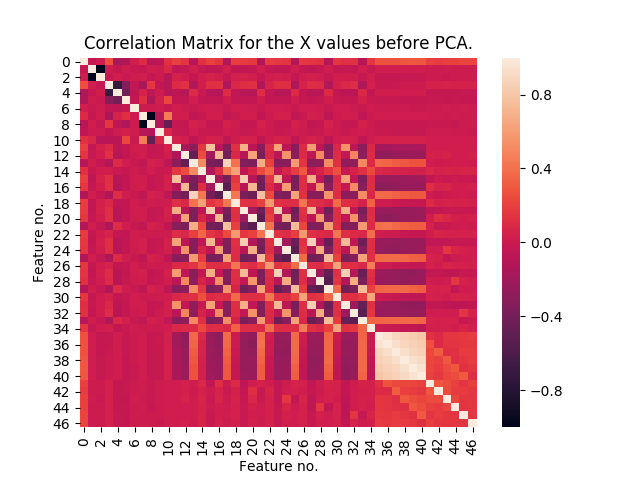
\includegraphics[width=0.5\textwidth]{figures/corr_pre-PCA.png}
                \caption{Correlation matrix heatmap before PCA was performed. }
                \label{fig:pre_PCA}
            \end{figure}
            It is clear here that there are many features that have linear dependencies. The goal is to diagonalize this such that all the features are linearly independent. This is why PCA was implemented. After the PCA was performed (with an eigenvalue limit of $\lambda > 0.1$), the features matrix looked like:
            \begin{figure}[H]
                \centering
                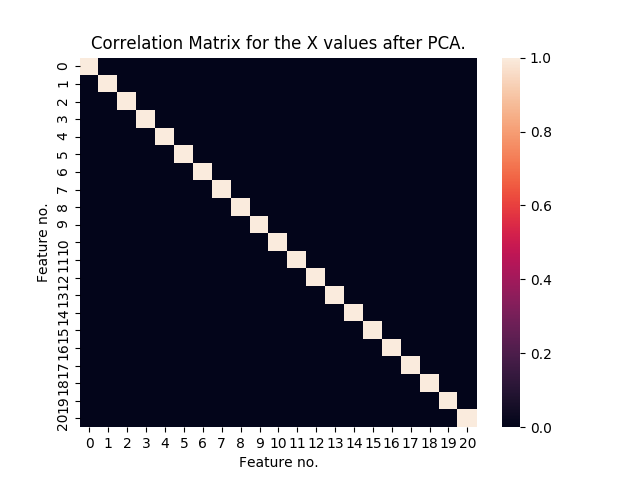
\includegraphics[width=0.5\textwidth]{figures/corr_post-PCA.png}
                \caption{Correlation matrix heatmap after PCA was performed. }
                \label{fig:post_PCA}
            \end{figure}
            This was the goal of the PCA. The features are now completely linearly independent of each other (correlation matrix is diagonalized), and the number of features is drastically reduced from 47 to 21. Now that the features are more computationally efficient and relevant, they can be input into the neural network system for training.
    
    \subsection{Neural Network Design}
        An object oriented code was built in Python 3.6.8 with the aim to make a generalized reusable code which has little to no specifications to the problem at hand. A large number of libraries are used for various different functionalities, the most important (excluding trivial unnecessary libraries) of them being:
        \begin{outline}[itemize]
            \1 NumPy version 1.17.2
                \2 NumPy is an excellent scientific programming library for handling of large array structures (e.g. matrix-matrix multiplication) and has a large number of useful built in functions (e.g. exponential and logarithm functions)
            \1 Pandas version 0.25.1
                \2 Pandas is primarily used for large data set manipulation and data processing. Several pandas functionalities are used when extracting and pre-processing the credit card data set.
            \1 Scikit-Learn version 0.21.3
                \2 Scikit-Learn (or sklearn) is a large library with a lot of useful functionality when it comes to regression and machine learning tasks. Many functions from sklearn are used throughout the study.
            \1 Matplotlib version 3.1.1
                \2 Matplotlib's PyPlot package is a Python library which is incredibly useful for data visualization and plotting. Several of the plots presented in this paper are generated by Matplotlib.
            \1 TensorFlow version 2.0.0
                \2 TensorFlow is Google's recently released machine learning library, and has an incredibly optimized neural network code structure. The network built using TensorFlow is therefore set to be a high benchmark for the neural network code built in this project.
            \1 Imbalanced-learn version 0.5.0
                \2 Imbalanced-learn (imblearn) is a package mainly used to up- and down-sample the data sets presented. The functionality of imblearn's package is quite easy to implement and is very time-efficient.
        \end{outline}
        Some packages implemented but left out of this list are Seaborn version 0.9.0 (used to produce the heatmaps illustrated in figures \ref{fig:pre_PCA} and \ref{fig:post_PCA}), Dill version 0.3.1.1 (used to save some trained neural network objects), and python utilities such as \textbf{os} (used for operating system functionality) and \textbf{time} (used to output the time taken to conduct calculations).
        
        \subsubsection{Weight- and Bias Initialization}
            Several different weight and bias initialization methods are implemented into the network class. The weights and bias initialization functions include the Xavier method introduced in equation \ref{eq:xavier}, a \textit{small} functionality, which initializes all weights and/or biases as $0.01$, and a \textit{random} functionality, initializing them using a random uniform distribution.
            
        \subsubsection{Hyperparameter and Learning Rate analysis}
            The simplest way of performing a search for the optimal parameters is initializing a grid search over multiple hyperparameter values $\lambda_i \in [\lambda_1, \lambda_2, \hdots, \lambda_{r1}]$ and learning rates $\eta_i \in [\eta_1, \eta_2, \hdots, \eta_{r2}]$, producing an array of $(r1 \times r2)$ trained neural networks. These networks must all have the same design to perform the analysis of $\lambda$ and $\eta$ properly.\\\\
            Several network designs are initialized with variations structures of hidden layers, node number per layer, activation function per layer, etc. The network structures researched were designed out of simple interest, where several of the networks are similar but have slight tweaks (such as increasing the number of nodes per layer by 10). This is done to research both the impact of the parameters $\lambda$ and $\eta$ simultaneously with the influence of other factors (such as the nodes per layer).
          
    \subsection{Classification}
        The goal of the classification research presented is to use the accuracy metric to compare the two methods of stochastic gradient descent and artificial neural network. A supplementary research study is conducted on the neural network, where an extensive search of which network structure produces the best results. The additional accuracy metrics of the area under the cumulative gain curve and $F1$ score are included for this study.
        \subsubsection{Logistic Regression}
            A class is built in python to perform the stochastic gradient descent presented in the theory section. several different initializing guesses $\hat{\beta}_0$ functionalities are included in this case, allowing for a custom guess to be passed in, or a request for the class to generate a random uniform distribution from $\hat{\beta}_i \in [-0.7, 0.7]$.
            % How did we set up LR?
                % Cost-function
                % SGD with mini-batched
                % Parameters used
                
        \subsubsection{Neural Network: Classification}
            The neural network code is implemented into an object oriented code in python, where several of the network attributes can be stored. There is also a large amount of functions implemented into the class which have various objectives, ranging from network training to network performance analysis. 
        
            % How did we set up NN?
                % appropriate COST-function: MSE or cross entropy
                % Vary "regularization parameters" and "learning rates" to find optimal accuracy
                    % We need an analysis of these two parameters
            
    \subsection{Regression}
        The goal of the regression research presented is use the mean-squared error $MSE$ cost function to compare the Ridge regression and neural network schemes. 
        \subsubsection{Linear Regression}
            The linear regression study conducted on Franke's function in this report is nearly identical to the study from our previous project. The code from that project is therefore utilized to produce results which are compared to the neural network. To see the details of the Ridge scheme code and the results of the project, visit the project 1 github page presented previously.
        \subsubsection{Neural Network: Regression}
            For the regression case, some additional functionalities needed to be added to the neural network class. This included changing the layout of the classes \textit{testing} function, as the parameters that are being tested are no longer the same (accuracy, area under curve, and $F1$ scores do not apply to regression cases). The way that the regression results are assessed is by the $MSE$ cost function presented previously. 